\subsection{Tag}
The tags is one of the core components of the program, as it allows the user to describe assets and their states and relations. In the system these are implemented from the interface \textit{ITagable}, this interface is implemented by the \textit{User} class (\autoref{ssc:Users}) as well as the \textit{Tag} class, as both of these can be tagged onto assets. \par
The \textit{Tag} class contains a label, \textit{Fields} and potentially a relation to a parent-tag. Parent tags are used to group tags, to make them easier to navigate and use. The relation between a parent and a child tag is a many to one relation stored in the database. \\
As seen on \autoref{fig:TagClass} the \textit{Tag} class contains the \textbf{Id}, \textbf{CreatedAt} and \textbf{UpdatedAt}, which are inherited from the \textit{Model} class, aside from this the \textit{Tag} class also contains a \textbf{FieldList}, a \textbf{Color} property and the Id of its parent. \par
The relation between an \textit{Asset} and a \textit{Tag} is defined in a relational database, containing the ID's of the connected tags and assets.

\begin{figure}[H]
    \centering
    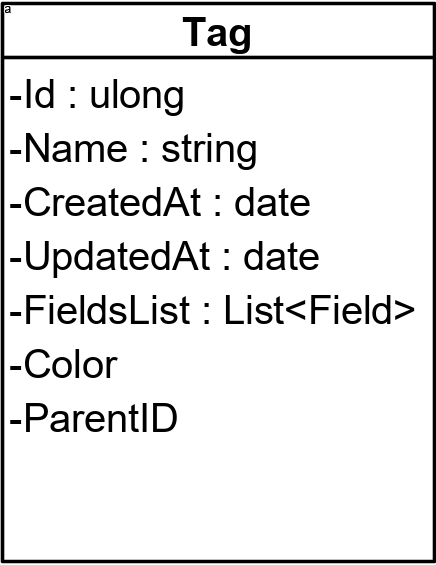
\includegraphics[width=0.2\textwidth]{figures/Implementation/Models/Tag.PNG}
    \caption{Tag class}
    \label{fig:TagClass}
\end{figure}



\subsubsection{User} \label{ssc:Users}
The \textit{User} class mostly functions as a \textit{Tag}, as it is tagged unto the assets on which it has a relation to. This takes the responsibility of the loan class mentioned in \autoref{ch:problemdomain}, hereby any generalized description of assets can be done via tags. \\
The user model contains the properties seen in \todo[inline]{Insert figure of User class}.